\chapter{Introduction}
\label{chap:Introduction}

Machine Learning (ML) is an area of computer science that provides the systems the ability to learn patterns and make deductions from it. Machine learning focuses on the development of computer programs (or algorithms) that can access data and use this data to learn salient features from it. ML algorithms are often categorized as supervised/unsupervised algorithms and reinforcement learning algorithms. 

Supervised algorithms learn from labelled training data and build a model out of it. The labelled data is a pair, consisting of an input value and a desired output value. Supervised algorithms analyse the training data and produce the output values. These output values are then used to map onto the desired output values to determine the performance of the model. In contrast, unsupervised learning looks for patterns in the dataset with minimum human supervision. The dataset does not contain any labels and the algorithms instead look for patterns.  

ML is also closely related to, and used in computational statics and data mining. Statistics and data mining can provide various analytical insights - descriptive, diagnostic, predictive, and prescriptive. 

Descriptive analytics is used to view existing data statistically which informs us about the past. This can provide the context to the dataset. Whereas, diagnostic analytics is used for cause analysis in a problem. This again is a pattern detection problem wherein ML can play an influential role. Predictive analytics is used for predicting an event from historical data. The historical data is used as an input to a machine learning model, which predicts the future event in a probabilistic method. Prescriptive analytics takes predictive analytics to a new step and suggests various courses of action and the potential implication of each action. 

For ML, one can also distinguish between training and inference phases. The dataset is divided accordingly into training, testing, and a validation dataset. In the training phase, the model tries to learn from the training dataset. If supervised learning is used, then the model learns to differentiate between various classes of data. The model predicts the class label and compares them to the actual labels. A validation dataset can be used to tune this model for producing better results. In the inference phase, this trained model is used to infer and predict for the testing dataset. This is usually the stage where this model is deployed to predict real-world data.

ML is used in a wide variety of applications. From virtual personal assistants to more industrial applications such as email filtering and computer vision, this field has improved the efficiency and consistency with which quality results are delivered.

Spurred by such high quality results and advances in processing power, memory, storage and an unprecedented wealth of data, the applications of ML are swiftly infiltrating many areas of the healthcare industry as well. From diagnosis and prognosis to drug development and epidemiology, machine learning has the potential to transform the medical landscape \cite{deo2015machine} \cite{beaulieu2019trends}. 

The increase in knowledge and understanding of diseases from numerous sources has provided a large source of information. This information can be used to tackle increasingly complex clinical tasks, often with astonishing success. A simple pipeline showcasing the use of such information is shown in Figure~\ref{fig:pipeline_clinical_care}. 

\begin{figure}[ht]
    \centering
    
\includegraphics[width=1.0\linewidth, height=6cm]{BachelorMasterThesis/Introduction/Figures/ml_pipeline_medicine.png}
    \caption{A simple pipeline for clinical care \cite{qayyum2020secure}}
    \label{fig:pipeline_clinical_care}
\end{figure}

The pipeline shows the development phase, where the data is collected through various sources and annotated. The annotated data is required in the training process for the model. The model as such, extracts features and does the classification task. This model can then be used to classify unknown data which becomes helpful to analyze, diagnose, and intervene to speed up the clinical process.

Machine learning has also become important in the medical field of electrocardiography, which deals in the process of producing an electrocardiogram (ECG) for heartbeats. ECG is a recording of the voltage of the electrical activity of the heart using electrodes, versus time. The normal rhythm of the heart is called sinus rhythm and this is necessary for normal electrical activity of the heart (Figure~\ref{fig:sinus_rhythm}). 

\begin{figure}[ht]
    \centering
    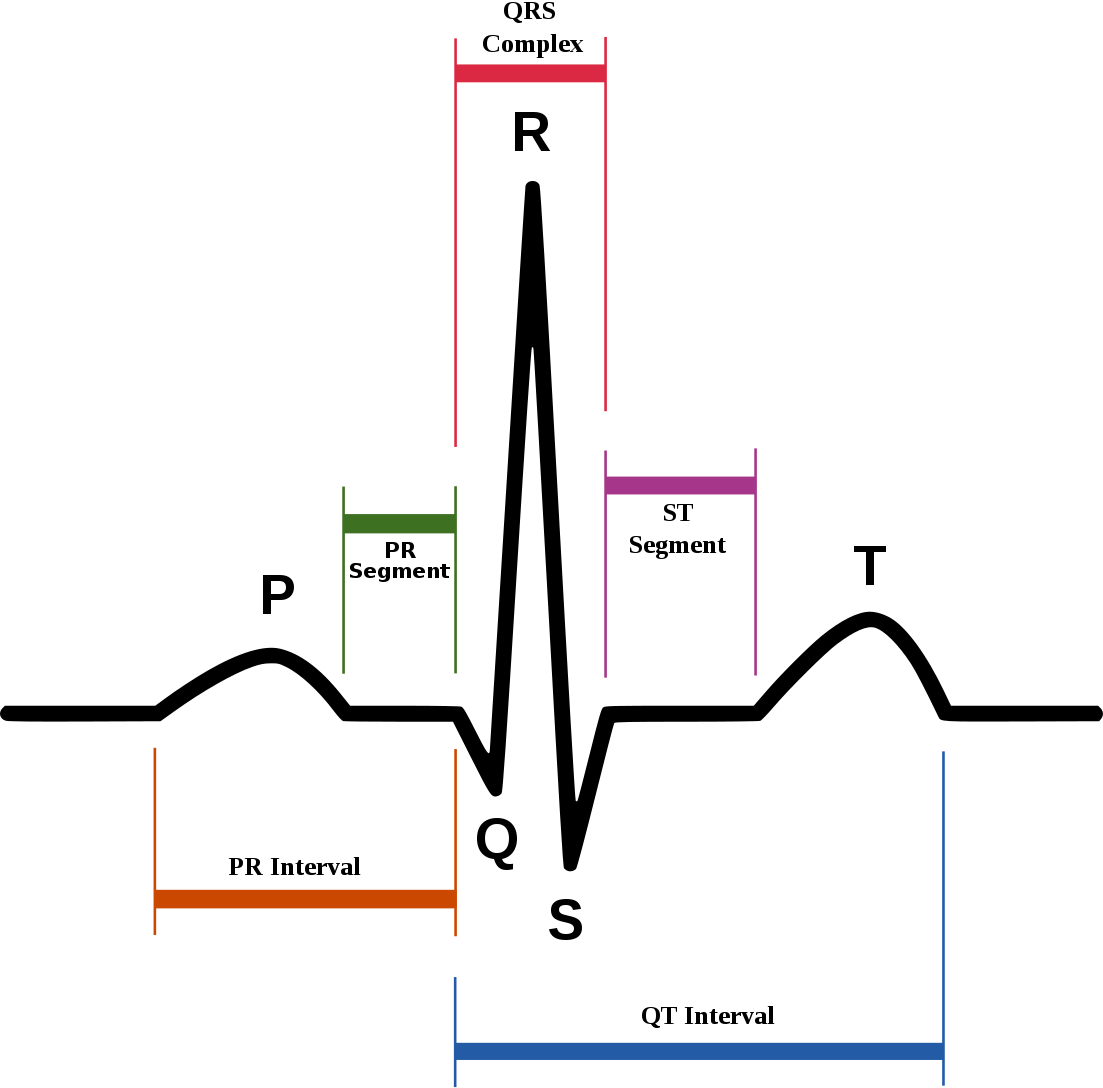
\includegraphics[width=0.6\linewidth, height=6.5cm]{BachelorMasterThesis/Introduction/Figures/SinusRhythmLabels.svg.png}
    \caption{ECG of a heart in normal sinus rhythm \cite{wiki:Electrocardiography}}
    \label{fig:sinus_rhythm}
\end{figure}

Changes in the normal ECG pattern are called cardiac abnormalities. The cases of these cardiac rhythm disturbances are called atrial fibrillation (AF) and ventricular tachycardia. "Tachyarrhythmia characterized by predominantly uncoordinated atrial activation with consequent deterioration of atrial mechanical function” is the definition coined by the American College of Cardiology (ACC), the American Heart Association (AHA) and the European Society of Cardiology (ESC) \cite{fuster2001acc} for atrial fibrillation.

Among the many cardiac disturbances, atrial fibrillation (AF) is  the most common cardiac arrhythmia \cite{smolen2017atrial} \cite{developed2010guidelines}. AF is associated with a high mortality rate and its detection is challenging as it may be episodic. Early detection of AF can be clinically significant to mitigate the risks caused by it. 

Deep learning (DL), a subclass of machine learning algorithms has shown high accuracy in performing pattern recognition for speech \cite{sak2014long}, image recognition \cite{russakovsky2015imagenet}, in detection of diabetic retinopathy \cite{gulshan2016development} and skin cancer \cite{esteva2017dermatologist}. 
Convolutional neural networks (CNNs) and Recursive neural networks (RNNs), a subset of DL, have achieved good results for ECG classification (Hannun et. al \cite{hannun2019cardiologist}) and can be used to detect AF.

\section{Problem Statement}
\label{sec:problem_statement}
State of the art deep neural networks (DNNs) for image classification commonly have a large number of parameters. For example, Inception-v3 \cite{szegedy2016rethinking} and ResNeXt-50 \cite{xie2017aggregated} architectures have about 25 million parameters, with the size of the models greater than 90MB. These are considerably large models with very high training times especially on conventional x86 central processing units (CPUs). 

To overcome this high training times, specialized hardware such as graphical processing units (GPUs), application specific integrated circuit (ASIC) and field programmable gate arrays (FPGAs) are designed. 
GPUs are commonly used hardware with a high parallel structure to enable high throughput. But because of the flexibility and ability to be re-configurable, the use of FPGAs is becoming increasingly common to train deep neural networks. FPGAs are also known to be more energy efficient when the classification pipelines grow \cite{qasaimeh2019comparing}.

With the development of such specialized hardware, research has been carried out into the field of energy efficiency. Energy-efficient hardware design requires a conscious consideration of the entire design space at various design levels, i.e at application, algorithm, architecture, and technology levels.
DNN models that are fairly large in size can become an obstacle to specialized hardware such as FPGAs and embedded devices. On such devices, DNNs should be optimized with regards to minimizing the number of operations required to perform a single classification action. This directly translates into the amount of energy consumed by the device.

Designing a new topology for such problems, with specific network constraints can be a difficult process. With the classical design strategy of trial and error, this is a cumbersome task as the search space is highly dimensional. A purely heuristic approach to solve this problem can be a time-consuming process. As such, evolutionary methods with genetic algorithms (AutoML approach) can be used to find an optimal network topology accommodating various network constraints.

Many network topologies can be analysed for the suitability of the problem whereas the optimal network structure depends on the goal to be achieved. The balance between multiple optimization criteria such as the number of parameters (which can be used to track energy consumption), the accuracy for the classification of the task, computational complexity, memory bandwidth of the hardware, and the memory requirement become essential. This approach with multiple objective functions to find a DNN topology by evolutionary means is the starting point for the project. 

\section{Our Contribution}

Keeping a holistic view of the problem, the main contribution of my work are as follows:

\begin{enumerate}
    \item Analyze electrocardiogram (ECG) data to examine if preprocessing is essential for the dataset.
    \item Develop baseline models (convolutional neural networks) to classify electrocardiogram (ECG) data.
    \item Develop an AutoML toolbox for topology search using evolution based methods with genetic algorithms for electrocardiogram (ECG) data.
    \item Add multiple selection strategies. 
    \item Extend the topology search to find a Pareto-optimal solution.
    \item Analyze various selection strategies and mutation policies. 
    % \item We analyze the effect of topology search combined with quantization (using TensorQuant \cite{loroch2017tensorquant}) to further minimize models that can be mapped efficiently on FPGAs.
    % \item We introduce a windowing approach to improve the speed of classification and to reduce the number of operations required to detect atrial fibrillation. 
\end{enumerate}

This work is integrated into a project which deals with the development of a generic AutoML toolbox. The optimization and implementation methods used in this project should be generic enough to be used for a wide variety of DL applications.
% , with minor adjustments in optimization parameters. 

\section{Structure of the report}

The report is divided into 7 chapters. After the introduction, the theoretical background of the various topics covered in the project is explained in \autoref{chap:theoretical_background}. This includes a theoretical explanation of convolutional neural networks (CNNs), deep neural networks (DNNs), DNNs for specialized hardware such as FPGAs and GPUs, the concepts of neural architecture search (NAS) and genetic algorithms for AutoML.

In \autoref{chap:related_work}, we speak about the various standard and state of the art approaches which have been attempted before for ECG signal classification in \autoref{sec:ecg_using_DNN}, deep neural networks for specialized hardware in \autoref{sec:DNN_for_specialized_hardware}, AutoML and neural architecture search approaches in \autoref{sec:autoML_NAS}.

In \autoref{chap:data_exploration}, we speak about data exploration. The description of the data in the dataset is pointed out in \autoref{sec:data_description}. The dataset is explored using various visualisation techniques in \autoref{sec:data_visulization} and a small analysis on the dataset in mentioned in the \autoref{sec:data_analysis} of that chapter. The seed models are discussed in \autoref{sec:seed_model}.

In \autoref{chap:approach_and_implementation}, we speak about the proposed approach for Auto-ML. The NAS pipeline used for classification is discussed in \autoref{sec:proposed_approach}. Encoding of layers is discussed in \autoref{sec:encoding_layers} where as in \autoref{sec:search_space} and \autoref{sec:fitness_evaluation}, the search space and fitness evaluation metrics are discussed respectively. The \autoref{sec:selection_strategy} speaks about the various selection strategies used in the thesis.

In \autoref{chap:experiments_and_results}, we discuss the results obtained from the various experiments conducted. The results in \autoref{sec:seed_model_experiments} are for the seed model where as \autoref{sec:nas_experiments} are for the NAS experiments. In \autoref{chap:conclusion_and_future_work}, we summarize the present work and discuss about the future work.

\afterpage{\blankpage}